%+++++++++++++++++++++++++++++++++++++++++++++++++++++++++++++++
% SUMMARY    : Introduction of Perceptron and the Hyperplane
%            : University of Southern Maine 
%            : @james.quinlan
%            : Mandy Ho - Lecture 6
%+++++++++++++++++++++++++++++++++++++++++++++++++++++++++++++++

\section*{Objectives}
\begin{outline}
    \1 Review KNN
    \2 Evaluating a model
    \1 The Perceptron Algorithm
\end{outline}
\rule[0.0051in]{\textwidth}{0.00025in}

% ----------------------------------------------------------------
\begin{center}
\begin{tikzpicture}
    \draw[very thin, gray] (-2.5,-2.5) grid (2.5,2.5);
    \draw[->, thick] (-2.6, 0) -- (2.6, 0) node[right] {$x$};
    \draw[->, thick] (0, -2.6) -- (0, 2.6) node[above] {$y$};

    % squares
    \foreach \x/\y in {0.2/0.4, 1.4/1.2, -0.8/0.2, 0.2/-0.3, -1.2/-0.1, -1.5/-0.9, -0.3/-0.2, 0.8/1.7} {
        \node[draw, fill=black, shape=rectangle, scale=0.8] at (\x,\y) {};
    }

    % circles
    \node[draw, fill=black, shape=circle, scale=0.6] at (0.9, -1.7) {};
    \node[draw, fill=black, shape=circle, scale=0.6] at (2.1, -0.3) {};
    \node[draw, fill=black, shape=circle, scale=0.6] at (-0.4, -2.1) {};

    % target
    \node[draw, fill=red, shape=star, star points=5, star point ratio=2.25, minimum size=12pt] at (0,0.7) {};
\end{tikzpicture}
\end{center}
% ----------------------------------------------------------------

\subsection*{1. K-Nearest Neighbors\cite{guo2003knn} (KNN) Review}
\begin{outline}
    \1 Pick $k$-nearest neighbors.
    \1 Easy, intuitive, and effective.
    \1 Not suitable for random data.
    \1 Assumptions:
        \2 There is a pattern to discern.
        \2 Computationally, the algorithm calculates distance, sorts, and selects $k$ nearest neighbors.
        \2 Data structures to facilitate this process include k-d trees and ball trees.
        \2 Example: Is the star a cat or a dog?
    \1 $k$ is a hyperparameter:
        \2 A hyperparameter is not learned or trained by the model.
        \2 You select the ``best" $k$ by tuning and training models on various different values of $k$.
        \2 Hyperparameter tuning methods:
            \3 \textbf{Cross-validation}: This method is used to measure how well a model performs on a dataset. Divide your dataset into subsets for training and validation/testing. Typically, cross-validation checks the average of multiple validation sets for a more accurate evaluation.
            \3 \textbf{Grid search}: Suppose you have two hyper-parameters, $a$ and $b$, that you want to train your model with. Define a grid with values of $a$ on one axis and values of $b$ on the other. The model then trains on each combination of $a$ and $b$ in the grid to determine the optimal combination. 
\end{outline}

\subsection*{Cross-Validation\cite{Kohavi1995ASO}}
\begin{outline}
    \1 What determines the split? The amount of data you have.
    \1 Most common split is 80/20, with 80\% of the dataset used for training and the remaining 20\% used for validation/testing. Other common splits are 70/30, 60/40, and 90/10. 
    \1 The more training data you have, the better the model performance.
\end{outline}



% ----------------------------------------------------------------
\begin{figure}[ht]
    \centering
    \begin{tikzpicture}[node distance=1.5cm and 2cm, auto]
        % Nodes
        \node (data) [draw, rectangle] {Data};
        \node (train) [below left=of data, draw, rectangle] {Training Set};
        \node (test)  [below right=of data, draw, rectangle] {Test Set};
        \node (dev)   [below left=of train, draw, rectangle] {Dev Set};
        \node (val)   [below right=of train, draw, rectangle] {Validation Set};
        \node (build) [below=of dev, draw, rectangle] {Develop, build, or train model};
        \node (train_all) [below=of val, draw, rectangle] {Train on everything};
        \node (final_test) [below=of train_all, draw, rectangle] {Finally test/retrain if test was good};
        
        % Arrows
        \draw[->] (data) -- (train);
        \draw[->] (data) -- (test);
        \draw[->] (train) -- (dev);
        \draw[->] (train) -- (val);
        \draw[->] (dev) -- (build);
        \draw[->] (val) -- (train_all);
        \draw[->] (build) -- (train_all);
        \draw[->] (train_all) -- (final_test);
        \draw[->, bend left=45] (test) to (final_test);
    \end{tikzpicture}
    \caption{Model Training Process}
    \label{fig:data_split_extended}
\end{figure}
% ----------------------------------------------------------------

\subsection*{Model Evaluation}
\vspace{0.5em}
How do we know whether a model is good? For classification models, we use the following metrics:

% ----------------------------------------------------------------
\begin{figure}[h]
    \centering
    \scalebox{0.7}{
        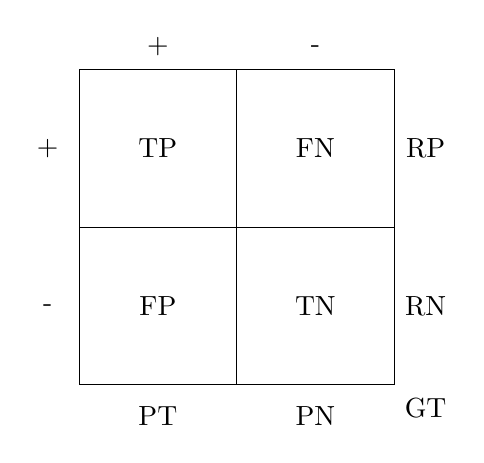
\begin{tikzpicture}
            \draw (0,0) rectangle (4,4);
            
            \draw (2,0) -- (2,4);
            \draw (0,2) -- (4,2);
            
            \node at (1,3) {TP};
            \node at (3,3) {FN};
            \node at (1,1) {FP};
            \node at (3,1) {TN};
            \node at (1,4.3) {+}; % Above TP
            \node at (3,4.3) {-}; % Above FN
            \node at (4.4,3) {RP}; % Beside FN
            \node at (4.4,1) {RN}; % Beside TN
            \node at (-0.4,3) {+}; % Left of TP
            \node at (-0.4,1) {-}; % Left of FP
            \node at (1,-0.4) {PT}; % Below FP
            \node at (3,-0.4) {PN}; % Below TN
            \node at (4.4,-0.3) {GT};
        \end{tikzpicture}
    }
    \caption{Confusion Matrix}
    \label{fig:confusion_matrix}
\end{figure}
% ----------------------------------------------------------------


\begin{outline}
    \1 \textbf{Accuracy}: The proportion of correct predictions. \(\frac{\text{TP} + \text{TN}}{\text{TP} + \text{FP} + \text{TN} + \text{FN}}\)
    \1 \textbf{Error Rate}: \(1 - \text{Accuracy} = \frac{\text{FP} + \text{FN}}{\text{GT}}\)
    \1 \textbf{Precision}: Measures how well the model classifies positives. \(\frac{\text{TP}}{\text{TP} + \text{FP}}\)
    \1 \textbf{Recall (Sensitivity)}: Measures how many positive instances were correctly predicted. \(\frac{\text{TP}}{\text{TP} + \text{FN}}\)
    \1 \textbf{Specificity}: Measures the proportion of true negatives correctly identified. \(\frac{\text{TN}}{\text{FP} + \text{TN}}\)
    \1 \textbf{F-Score}: The harmonic mean of precision and recall. Best when \(B = 1\).
\end{outline}

\subsection*{2. Perceptron Algorithm}

\begin{outline}
    \1 First machine learning/AI algorithm, introduced by Frank Rosenblatt in 1957 at Cornell University\cite{rosenblatt1958perceptron}.
    \1 The goal is to find a decision boundary or hyperplane to separate the data. There can be multiple decision boundaries.
    \1 For non-linear decision boundaries, techniques like the kernel trick can be used to create a hyperplane.

    \1\textbf{Kernel Trick:} The kernel trick enables the perceptron to operate in higher-dimensional spaces by replacing the standard dot product with 
    a kernel function. This kernel function effectively computes the dot product in a transformed, higher-dimensional space without 
    explicitly performing the transformation. It acts as a similarity measure between points, corresponding to a dot product in that 
    space. The trick works because the perceptron decision function is based solely on dots between data points. By substituting a kernel 
    function, the perceptron can classify data in a higher-dimensional space, where it might become linearly separable, without the computational 
    expense of transforming the points directly.
 
    \1 Assumptions:
    
        \2 The data is linearly separable.
    \1 Definition: Hyperplane
    
        \2 $\{(\vec{x}_1,y_1),(\vec{x}_2,y_2),...,(\vec{x}_n,y_n)\}$ where $y$ are labels.
        \2 $\mathcal{H}=\{x_i\mid w^Tx+b=0\}$ where $w$ is the vector of weights and $b$ is the bias and $b\in\mathbb{R}$.
        \2 Goal is to find $w$ and $b$.

    \1 Code example of perceptron:
    \begin{minted}[fontsize=\small]{python}
def perceptron(D, max_epochs=100):
    """
    Perceptron algorithm for binary classification.

    Input:
    - D: Training dataset, a list of tuples (x_i, y_i), where x_i is the feature vector 
         and y_i is the label (-1 or 1).
    - max_epochs: Maximum number of iterations over the dataset.

    Output:
    - w: Learned weight vector (including bias term).
    """
    
    # Step 1: Initialize weight vector and bias to zero
    n_features = len(D[0][0])  # Number of features in x_i
    w = [0.0] * n_features  # Weight vector
    b = 0.0  # Bias term
    
    # Step 2: Initialize misclassification counter
    m = 1  # Assume at least one misclassification
    
    # Step 3: Iterate until no misclassifications or max_epochs reached
    epoch = 0
    while m > 0 and epoch < max_epochs:
        m = 0  # Reset misclassification counter
        
        # Step 5: Iterate over all training examples
        for x_i, y_i in D:
            # Step 6: Check if the example is misclassified
            # Compute the dot product w · x_i, add bias, and check if y_i * (w · x_i + b) <= 0
            if y_i * (sum(w[j] * x_i[j] for j in range(n_features)) + b) <= 0:
                # Step 7: Update weight vector and bias
                for j in range(n_features):
                    w[j] += y_i * x_i[j]
                b += y_i
                m += 1  # Increment misclassification counter
        
        epoch += 1
    
    # Bundle weights and bias into a single vector
    w.append(b)  # Append bias as the last element of w
    return w
\end{minted}
    
\end{outline}


\begin{outline}
    \1 First machine learning/AI algorithm, introduced by Frank Rosenblatt in 1957.
    \1 The goal is to find a decision boundary or hyperplane to separate the data. There can be multiple decision boundaries.
    \1 For non-linear decision boundaries, techniques like the kernel trick can be used to create a hyperplane.
    \1 Assumptions:
        \2 The data is linearly separable.
    \1 Definition: Hyperplane
        \2 $\{(\vec{x}_1,y_1),(\vec{x}_2,y_2),...,(\vec{x}_n,y_n)\}$ where $y$ are labels.
        \2 $\mathcal{H}=\{x_i\mid w^Tx+b=0\}$ where $w$ is the vector of weights and $b$ is the bias and $b\in\mathbb{R}$.
        \2 Goal is to find $w$ and $b$.
\end{outline}


\section{Exploration (XPL) Problems}
\begin{outline}[enumerate]

    \1  Is it possible to have 100\% Sensitivity? \\
    \1  For multiple values of $\beta$, determine $\beta$'s effect on the $F_\beta$ score.\\

\end{outline}
